\documentclass{article}

% if you need to pass options to natbib, use, e.g.:
\PassOptionsToPackage{numbers, compress}{natbib}
% before loading neurips_2024

% ready for submission
%\usepackage{neurips_2024}

% to compile a preprint version, e.g., for submission to arXiv, add add the
% [preprint] option:
\usepackage[preprint]{neurips_2024}

% to compile a camera-ready version, add the [final] option, e.g.:
%     \usepackage[final]{neurips_2024}

% to avoid loading the natbib package, add option nonatbib:
%    \usepackage[nonatbib]{neurips_2024}

\usepackage[utf8]{inputenc} % allow utf-8 input
\usepackage[T1]{fontenc}    % use 8-bit T1 fonts
\usepackage{hyperref}       % hyperlinks
\usepackage{url}            % simple URL typesetting
\usepackage{booktabs}       % professional-quality tables
\usepackage{amsfonts}       % blackboard math symbols
\usepackage{nicefrac}       % compact symbols for 1/2, etc.
\usepackage{microtype}      % microtypography
\usepackage{xcolor}         % colors

\usepackage{comment}
\usepackage{csquotes}

\usepackage{tikz}
\usetikzlibrary{positioning,arrows.meta,fit,backgrounds}

% boolean options to add acknowledgements or combine main document with supplemental materials document
\usepackage{ifthen}

% reset counters for pages, figures, and tables in supplemental materials
\newcommand{\beginsupplement}{%
        \setcounter{table}{0}%
        \renewcommand{\thetable}{S\arabic{table}}%
        \setcounter{figure}{0}%
        \renewcommand{\thefigure}{S\arabic{figure}}%
        \setcounter{equation}{0}%
        \renewcommand{\theequation}{S\arabic{equation}}%
        \setcounter{section}{0}%
        \renewcommand{\thesection}{S\arabic{section}}%
        \setcounter{page}{1}%
        \renewcommand{\thepage}{S\arabic{page}}%
}

\newcommand{\ck}[1]{\textcolor{cyan}{CK: #1}}

\title{Spaced-Replay Continual Finetuning: Predicting Forgetting and Scheduling Adaptive Replay in Large Language System}

\author{%
  Minh Nguyen\thanks{This project is for the CSC 447 course at the University of Rochester.}\\
  Ngoc Mai Pham\thanks{This project is for the CSC 447 course at the University of Rochester.} \\
  Department of Computer Science\\
  University of Rochester\\
  \texttt{mnguy31@ur.rochester.edu}\\
  \texttt{mpham8@u.rochester.edu}
}

\begin{document}

\maketitle

\begin{abstract}
Catastrophic forgetting remains a fundamental obstacle for AI systems in general and LLM-system specifically trained on non\mbox{‑}stationary data streams.  Although experience replay buffers reduce forgetting, they scale poorly and often rely on naive sampling.  Inspired by cognitive science, where spaced practice and forgetting curves guide review schedules, we propose to study continual finetuning under limited compute and memory.  The project seeks to (i) measure sample\mbox{‑}level forgetting curves during sequential finetuning and (ii) design spacing\mbox{‑}inspired replay policies that predict when each sample or concept is at risk of being forgotten using uncertainty, gradient norms, loss trajectories and representation drift.  We will evaluate whether adaptive spaced replay on small models can deliver better long\mbox{‑}term retention than existing baselines with the same memory and limited compute budget.
\end{abstract}

%%%%%%%%% BODY TEXT
\section{Introduction}
\label{sec:intro}

Continual learning (CL) aims to endow neural networks with the ability to accumulate knowledge over a sequence of tasks without catastrophic forgetting.  Most deep networks are trained in a static, one\mbox{‑}shot setting and struggle to maintain performance when exposed to non\mbox{‑}IID data streams \citep{aljundi2019mir}; the stability and plasticity trade\mbox{‑}off is still an open challenge \citep{delange2021survey, wang2024comprehensive, chaudhry2019tiny}.  Rehearsal\mbox{‑}based methods, such as Experience Replay (ER), alleviate forgetting by maintaining a buffer of past examples and interleaving them with new data \citep{chaudhry2019tiny}.  While effective, these methods typically rely on random sampling and require large buffers to guarantee good coverage, which is impractical for resource\mbox{‑}constrained devices.

In contrast, cognitive psychology has long demonstrated that spaced retrieval practice, the art of reviewing material at increasing intervals, produces durable and long=lasting learning and reduces the need for massed review \citep{cepeda2008spacing}.  Complementary learning systems theory posits that rapid encoding (hippocampus) and slow neocortical consolidation rely on replay of old memories to integrate new knowledge without interference \citep{mcclelland1995cls}.  Recent CL research has begun to explore representation drift \citep{caccia2022ace, theofilou2025stabledrift}, gradient interference \citep{aljundi2019mir}, uncertainty\mbox{‑}based sample selection \citep{serra2025uncertainty}, and learning\mbox{‑}speed\mbox{‑}based signals \citep{hacochen2025sbs} to prioritize which data point to be retrained.  However, to the best of the author's extend, these techniques have not explicit target and utilize forgetting curves or the temporal spacing of the retrain data point.

\textbf{Scope.}  
This project focuses on \emph{continual finetuning}: the stage where a pretrained model is sequentially adapted to downstream tasks or domains \citep{wang2024comprehensive}.  We restrict ourselves to moderately sized models (i.e ResNet\mbox{‑}18 or DistilBERT) that can be trained efficiently on an Apple M3 Pro laptop.  Rather than pursuing generative replay, we assume access to a bounded buffer and investigate whether sample\mbox{‑}level signals can predict future forgetting under a non\mbox{‑}IID streams.  We further propose to schedule replay sessions using a spacing rule: revisit each sample just before its predicted forgetting time, thus, we can minimize the computation while maximizing data retention.

\paragraph{If successful, this work will make the following major contributions:}
\begin{enumerate}
    \item We introduce a methodology to measure \emph{forgetting curves} of individual samples and concepts during continual finetuning, characterizing how loss, confidence, and representations decay over time.
    \item We evaluate the four predictive signals of uncertainty, gradient norms, loss trajectories and representation drift to assess their ability to forecast imminent forgetting.
    \item We propose a spaced\mbox{‑}replay scheduler that adapts the replay interval of each memory based on predicted forgetting times and demonstrate improved accuracy and memory utilization on image and language benchmarks under fixed buffer and compute budgets.
    \item We provide an open\mbox{‑}source implementation and analysis of continual finetuning on Apple hardware, thus, highlighting practical considerations when designing CL algorithms for edge devices with limited capabilities.
\end{enumerate}

\begin{figure}[t]
\centering
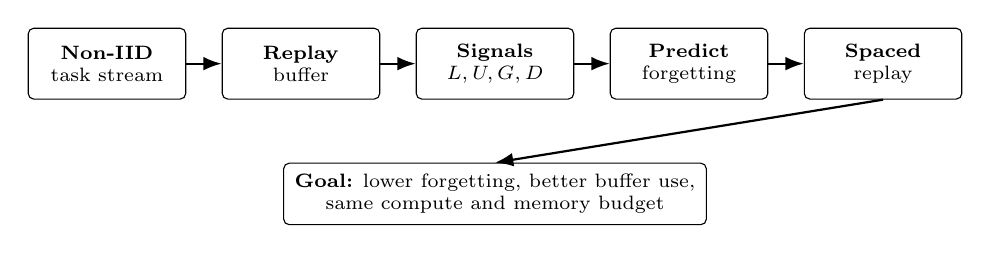
\begin{tikzpicture}[
    font=\scriptsize,
    >=Latex,
    node distance=0.55cm and 0.45cm,
    box/.style={
        draw,
        rounded corners=2pt,
        align=center,
        minimum width=2.0cm,
        minimum height=0.9cm,
        inner sep=4pt
    },
    arrow/.style={->, thick}
]
\node[box] (stream) {\textbf{Non-IID}\\task stream};
\node[box, right=of stream] (buffer) {\textbf{Replay}\\buffer};
\node[box, right=of buffer] (signals) {\textbf{Signals}\\$L,U,G,D$};
\node[box, right=of signals] (pred) {\textbf{Predict}\\forgetting};
\node[box, right=of pred] (sched) {\textbf{Spaced}\\replay};

\draw[arrow] (stream) -- (buffer);
\draw[arrow] (buffer) -- (signals);
\draw[arrow] (signals) -- (pred);
\draw[arrow] (pred) -- (sched);

\node[draw, rounded corners=2pt, below=0.8cm of signals, align=center, inner sep=4pt] (out) {
\textbf{Goal:} lower forgetting, better buffer use,\\same compute and memory budget
};
\draw[arrow] (sched.south) -- (out.north);
\end{tikzpicture}
\caption{Spaced-replay continual finetuning: monitor replay-buffer samples, predict when they will be forgotten, and replay them just before failure.}
\label{fig:compact_visual_abstract}
\end{figure}

\section{Background}
\label{sec:background}
\textbf{Continual Learning (CL).}
Continual learning is a well-established paradigm within the field of Artificial Intelligence. It is characterized by enabling AI models that are trained on static content and datasets to have the ability to learn new information, new events, and new knowledge that did not exist within their training data before, often from non-IID data streams in which incoming samples arrive sequentially and do not follow a single fixed shuffled distribution \citep{wang2024comprehensive}. Such forgetting can be studied at the sample level, where individual examples are tracked, or at the concept level, where groups of related samples such as classes or semantic clusters are monitored together.   

\textbf{Experience replay and representation drift.}  
A baseline for continual learning (CL) is to store a small subset of previous data and jointly train on current and buffered samples \citep{chaudhry2019tiny}.  Despite its simplicity, ER often outperforms more complicated regularization\mbox{‑}based approaches \citep{delange2021survey}.  However, ER does not explicitly mitigate \emph{representation drift} (or \emph{latent drift} per New
insights on reducing abrupt representation change in online continual learning): when new classes arrive, latent features for older classes shift, causing data to overlap and accuracy overall to degrade \citep{caccia2022ace}.  Methods such as ACE protects the old representations by using asymmetric updates, while ESMER models error sensitivity and selects low\mbox{‑}loss samples to reduce drift \citep{sarfraz2023esmer}.  Latent\mbox{‑}drift replay strategies further propose selecting slices with maximal internal feature shift to prioritise for rehearsal \citep{theofilou2025stabledrift}.

\textbf{Sample selection signals.}  
Several works propose signals for choosing which memories to replay.  Maximally interfered retrieval (MIR) estimates how much a sample's loss would increase given an upcoming parameter update and retrieves samples with highest gradient interference \citep{aljundi2019mir}.  Predictive uncertainty has been explored as a measure of a sample's position in decision space; uncertainty\mbox{‑}based selection can reduce forgetting when combined with a small buffer \citep{serra2025uncertainty}.  Speed\mbox{‑}based sampling observes that examples learned quickly are less prone to forgetting and selects samples based on learning speed \citep{hacochen2025sbs}.  These studies basically all implicitly hint at the existence of a forgetting curves, but none of the studies explicitly model or forecast when a sample will fail.

\textbf{Spacing and complementary learning systems.}  Cognitive science shows that spaced practice, the art of reviewing material after a delay, often leads to better longterm retention compared to massed practice \citep{cepeda2008spacing}.  Optimal spacing intervals depend on the desired retention time: subsequent reviews should occur when retrieval becomes effortful but before the memory is lost.  The complementary learning systems theory provides a neurobiological account: fast hippocampal encoding and slow neocortical consolidation rely on replay of old memories interleaved with new experiences to avoid interference \citep{mcclelland1995cls}.  Our work seeks to bring these insights into the design of replay buffers for continual finetuning.

\textbf{Generative replay and taxonomies.}  Generative replay approaches use a generator (for example, GAN or diffusion model) to synthesise past data instead of storing raw samples.  Recent diffusion\mbox{‑}based methods (DDGR) use a diffusion generator with an instruction operator to avoid drift \citep{gao2023ddgr}, and conditional diffusion replay has been extended to federated learning \citep{mei2024dcfl}.  These works aim at large\mbox{‑}scale settings but are computationally heavy and beyond our scope.  Comprehensive taxonomies of catastrophic forgetting classify methods into replay\mbox{‑}based, regularisation and parameter isolation families and highlight gaps \citep{aleixo2023taxonomy}.  Weight regularisation techniques like EWC measure parameter importance via the Fisher information matrix but suffer from gradient vanishing; recent work proposes logit reversal to improve EWC \citep{liu2026ewcdr}.  Our focus on replay complements these efforts by exploring spacing and forgetting prediction.

\section{Approach}

We frame continual finetuning as a stream of tasks $\{\mathcal{D}_1, ..., \mathcal{D}_T\}$.  At time $t$, the model parameters $\theta_t$ are updated by gradient descent on the current minibatch and a sample from the replay buffer $\mathcal{B}$.  Each buffered example $i$ is associated with four signals measured during training:

\begin{itemize}
    \item \textbf{Loss trajectory} $L_i(t)$: the cross\mbox{‑}entropy loss of sample $i$ evaluated periodically during training.  We normalise and smooth the trajectory to estimate the rate of loss increase; rising loss signals potential forgetting.
    \item \textbf{Uncertainty} $U_i(t)$: we compute predictive entropy or margin on sample $i$.  Lower confidence than at the time of learning indicates the model is becoming uncertain about the correct label.
    \item \textbf{Gradient norm} $G_i(t)$: we compute the $\ell_2$ norm of the gradient $\nabla_{\theta} \ell(x_i,y_i)$ without updating parameters.  A large gradient norm suggests that retaining this sample would require a significant parameter change, implying it is being forgotten.
    \item \textbf{Representation drift} $D_i(t)$: for one or two hidden layers, we measure the cosine distance between the activation vector at time of insertion $h_i(t_0)$ and its current activation $h_i(t)$.  High drift indicates that the internal representation of the sample has moved.
\end{itemize}

\subsection{Predicting forgetting}
For each sample, we define a binary target variable $\delta_i(t)$ indicating whether the sample will be forgotten within a fixed future horizon $\tau$ (i.e, it becomes misclassified or its loss increases beyond a threshold).  We collect a dataset of feature vectors $(L_i(t), U_i(t), G_i(t), D_i(t))$ and corresponding targets by monitoring the buffer during finetuning.  We will fit linear regession, logistic regression, support-vector machine and/or gradient boosting models to predict $\delta_i(t)$, and evaluate precision–recall on held\mbox{‑}out streams.  We will also experiment with concept\mbox{‑}level aggregation by grouping samples by class or semantic cluster and/or predicting group forgetting.

\subsection{Spacing replay scheduler}
Given a predictor that outputs the probability of forgetting within $\tau$, we derive a sample\mbox{‑}specific review interval.  From which, we can compute an estimated forgetting time $\hat{T}_i$ from the function and schedule the next replay at $t + \hat{T}_i$.  When the buffer is full, we shall prioritise samples with highest forgetting probability: Those with low forgetting risk can have their replay delayed or freeing capacity for new data.  We will compare simple heuristics (maybe sample once every $k$ iterations and random selection) to our adaptive scheduler.

\section{Experiments}
We will evaluate our approach on standard CL benchmarks adapted for continual finetuning.  For images, we will use Split CIFAR\mbox{‑}100 and Split CUB. For language, if time permits, we will use sequential domain adaptation of a pretrained DistilBERT on sentiment datasets.  Each task contains distinct classes or domains, and we treat each domain sequentially.  Models are initialised from a publicly available pretrained network.  We will implement ER, MIR, ESMER and uncertainty\mbox{‑}based baselines and compare them with our spaced\mbox{‑}replay scheduler.

\paragraph{Evaluation metrics.}  We will report final accuracy on all tasks, average forgetting (difference between best and last performance), computational cost (training time per task) and buffer utilisation (replay operations per iteration).  For each predictive signal, we will measure the area under the precision-recall curve of the forgetting predictor and ablate its contribution to the scheduler.

\subsection{Computational Resources}
Our experiments will run on a MacBook Pro equipped with an Apple M3 Pro System\mbox{‑}on\mbox{‑}Chip (12\mbox{‑}core CPU with 6 performance and 6 efficiency cores, 18\mbox{‑}core GPU and 36\,GB of unified memory).  We will use PyTorch's Metal backend to leverage the integrated GPU.  To fit within memory constraints, we will restrict models to \texttt{ResNet\mbox{‑}18} for vision and \texttt{DistilBERT} for language, use half\mbox{‑}precision training, and limit the replay buffer to a few hundred samples.  Preliminary profiling shows that training on Split CIFAR\mbox{‑}100 with a 200\mbox{‑}sample buffer completes in under two hours on this hardware, thus, suggesting that the proposed experiments are feasible.

\section{Timeline}
\begin{itemize}
    \item \textbf{Week 1-2:} Reproduce Experienced Replay (ER) baseline on Split CIFAR\mbox{‑}100 and collect initial forgetting curves.  Implement logging of loss, uncertainty, gradient norm and representation drift.
    \item \textbf{Week 3:} Train predictive models for sample\mbox{‑}level forgetting on collected data.  Explore concept\mbox{‑}level aggregation.  Conduct ablation to assess individual signals.
    \item \textbf{Week 4:} Implement spacing\mbox{‑}inspired replay scheduler.  Integrate forgetting predictors into buffer management.  Benchmark against MIR, uncertainty\mbox{‑}based and random sampling baselines. Conduct additional experiments with language models if time permits.
    \item \textbf{Week 5:} Prepare final report, including analysis of forgetting curves, predictor performance, and scheduling benefits.  Submit report.
\end{itemize}

%References
{\small
\bibliographystyle{ieee_fullname}
\bibliography{library}
}

\end{document}
